\documentclass[a4paper, 10pt]{article}
\usepackage{pgfplots} % Used for plotting functions

\pgfplotsset{compat=1.18} % Add this line to set the compatibility version


\usepackage[margin = 1in]{geometry} % for spacing around
\usepackage{graphicx} % for including images in your pdfs
\usepackage{xcolor} % for including colors in your pdf
\usepackage{soul} % for text decoration
\usepackage[utf8]{inputenc} % for encoded text
\usepackage[T1]{fontenc}
\usepackage{setspace} % for setting different line spacings between paragrafs.
\usepackage{enumerate} % for letting us get more detailed enumerate lists
\usepackage{multirow} % to let us combine more rows together
\usepackage{colortbl} % for decorating tables
\usepackage{amsmath} % used for representing more complicated math displays
\usepackage{supertabular}
\usepackage{longtable} % both of these packages are used to making really big tables
\usepackage{wrapfig} % allows us to wrap text around figures
\usepackage{fancyhdr} % for making fancy headers
%\usepackage{bibtex} % for making better bibliographies
\usepackage[pdftex]{hyperref} % for letting us make links
\usepackage{lscape} % Allows us to flip from portrait to landspace
\usepackage{tikz} % for high detailed drawing
\usepackage{multicol} % To put things side by side
\usepackage{rotating} % For rotating objects
% \usepackage{draftwatermark} % For adding watermarks
\usepackage{MnSymbol} % for using multiple symbols
\usepackage{mathtools} % Used for more math symbols
\usepackage{xfrac} % For more complciated fractions and to add derivitives
\usepackage{hyperref} % for hyper links
\usepackage{enumitem} % for better enum lists
\usepackage{tcolorbox} % for adding colored text boxes
\usepackage{bm} % Adding bold text to math inputs
\usepackage{pgfplots} % Used for plotting functions
\usepackage{booktabs} % For prettier tables
\usepackage{subcaption} % For subfigures
\usepackage{siunitx} % Add the siunitx package for number column alignment

% Setting up the default image path
\graphicspath{{../../global-assets/images/}}

% Implementing authro details
\title{Lab Report number I - Title of the lab report\\
	ENS203 - Electrical Circuits I}
\author{Emre Arapcic-Uevak\\220302289}
\date{}

% Setting up the fancy page style
\fancypagestyle{customStyle}{
	\lhead{} \chead{} \rhead{}
	\lfoot{} \cfoot{\thepage} \rfoot{}
	\renewcommand{\headrulewidth}{0pt}
	\renewcommand{\footrulewidth}{1pt}
}
\pagestyle{customStyle}

% Custom commands

\begin{document}
	\begin{titlepage}
		\begin{center}
			\vspace*{\stretch{1}} % Add vertical space before the title

			{\Large\bfseries Lab Report number 5 \\[0.5em] Wheatstone Bridge\par}
			\vspace{1cm} % Space between title and course title

			{\large ENS203 – Electrical Circuits I\par}
			\vspace{1cm} % Space between course title and your name/ID

			{\large Emre Arapcic-Uevak \\ 220302289\par}
			\vspace{1cm} % Space between your name/ID and assistant name

			{\large Afan Haznadarevic \\ 220302128\par}
			\vspace{.5cm} % Space between your name/ID and assistant name

			{\large Assistant: Adil Hasanbasic\par}
			\vspace{\stretch{2}} % Variable vertical space between assistant name and bottom
			
\includegraphics[width=0.5\textwidth]{Logo.png}
			\vspace{5mm}
			
			\textsc{\LARGE Internation University of Sarajevo}\\[1.5cm]
			\textsc{\Large ENS203 - Electrical Circuits I}\\[0.5cm]
			
			\rule{\linewidth}{0.5mm} \\[0.4cm]
			{ \huge \bfseries Lab Report number V - Wheatstone bridge}\\[0.4cm]
			\rule{\linewidth}{0.5mm} \\[1.5cm]
			
			\vfill
			
			% Bottom of the page
			{\large \today}
		\end{center}
	\end{titlepage}
	\pagebreak

	\tableofcontents
	\pagebreak
	
	\listoffigures
	\pagebreak

	\listoftables	
	\pagebreak 
	
	\section{Objective}
		\subsection{Wheatstone}
			\begin{figure}[h!]
				\centering
				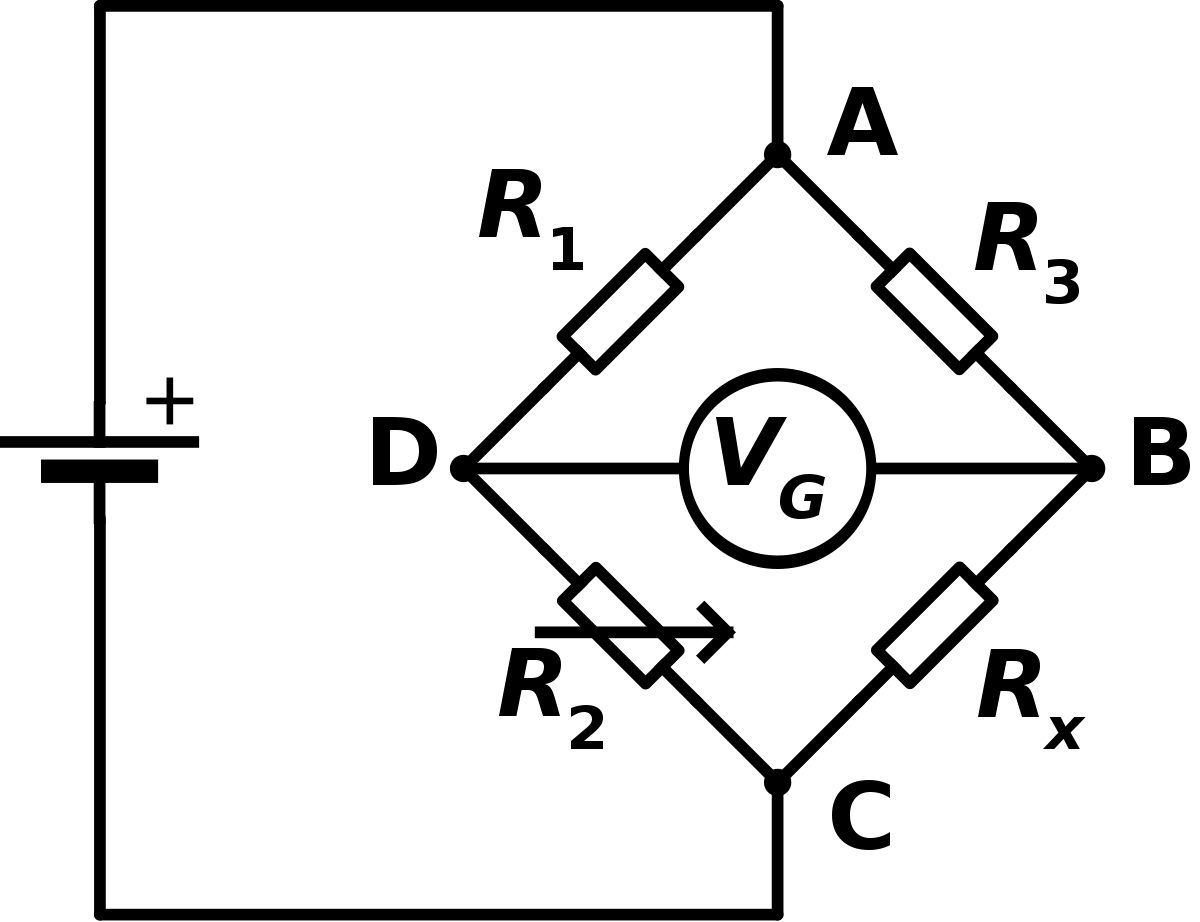
\includegraphics[width=0.5\textwidth]{./images/WheatstoneBridge.png}
				\caption{Wheatstone Bridge}
				\label{fig:wheatstone}
			\end{figure}

			The wheatstone bridge is a circuit that is used to measure an unknown resistance. 
			The circuit consists of four resistors, two of which are known, 1 variable resistor, and 1 unknown resistor.
			The circuit is balanced when the voltage between the two nodes is zero. 
			When the circuit is balanced, the ratio of the two known resistors is
			equal to the ratio of the two unknown resistors, or in other words 
			\begin{equation}
				\frac{R_1}{R_2} = \frac{R_3}{R_x}
			\end{equation}
			then we know that $V_D = V_B$, so the potential difference between the two nodes, $V_{DB}$, is zero.

			In today's lab, we will be using the wheatstone bridge and a multimeter to see when the bridge
			is balanced.

		\subsection{Apparatus}
			\begin{itemize}
				\item Multimeter
				\item Potenciometer
				\item Resistors
				\item DC Power Supply
				\item Breadboard
			\end{itemize}

			\pagebreak
			\subsubsection{DC Power Supply}
				Used to provide a constant voltage
				\begin{figure}[h!]
					\centering
					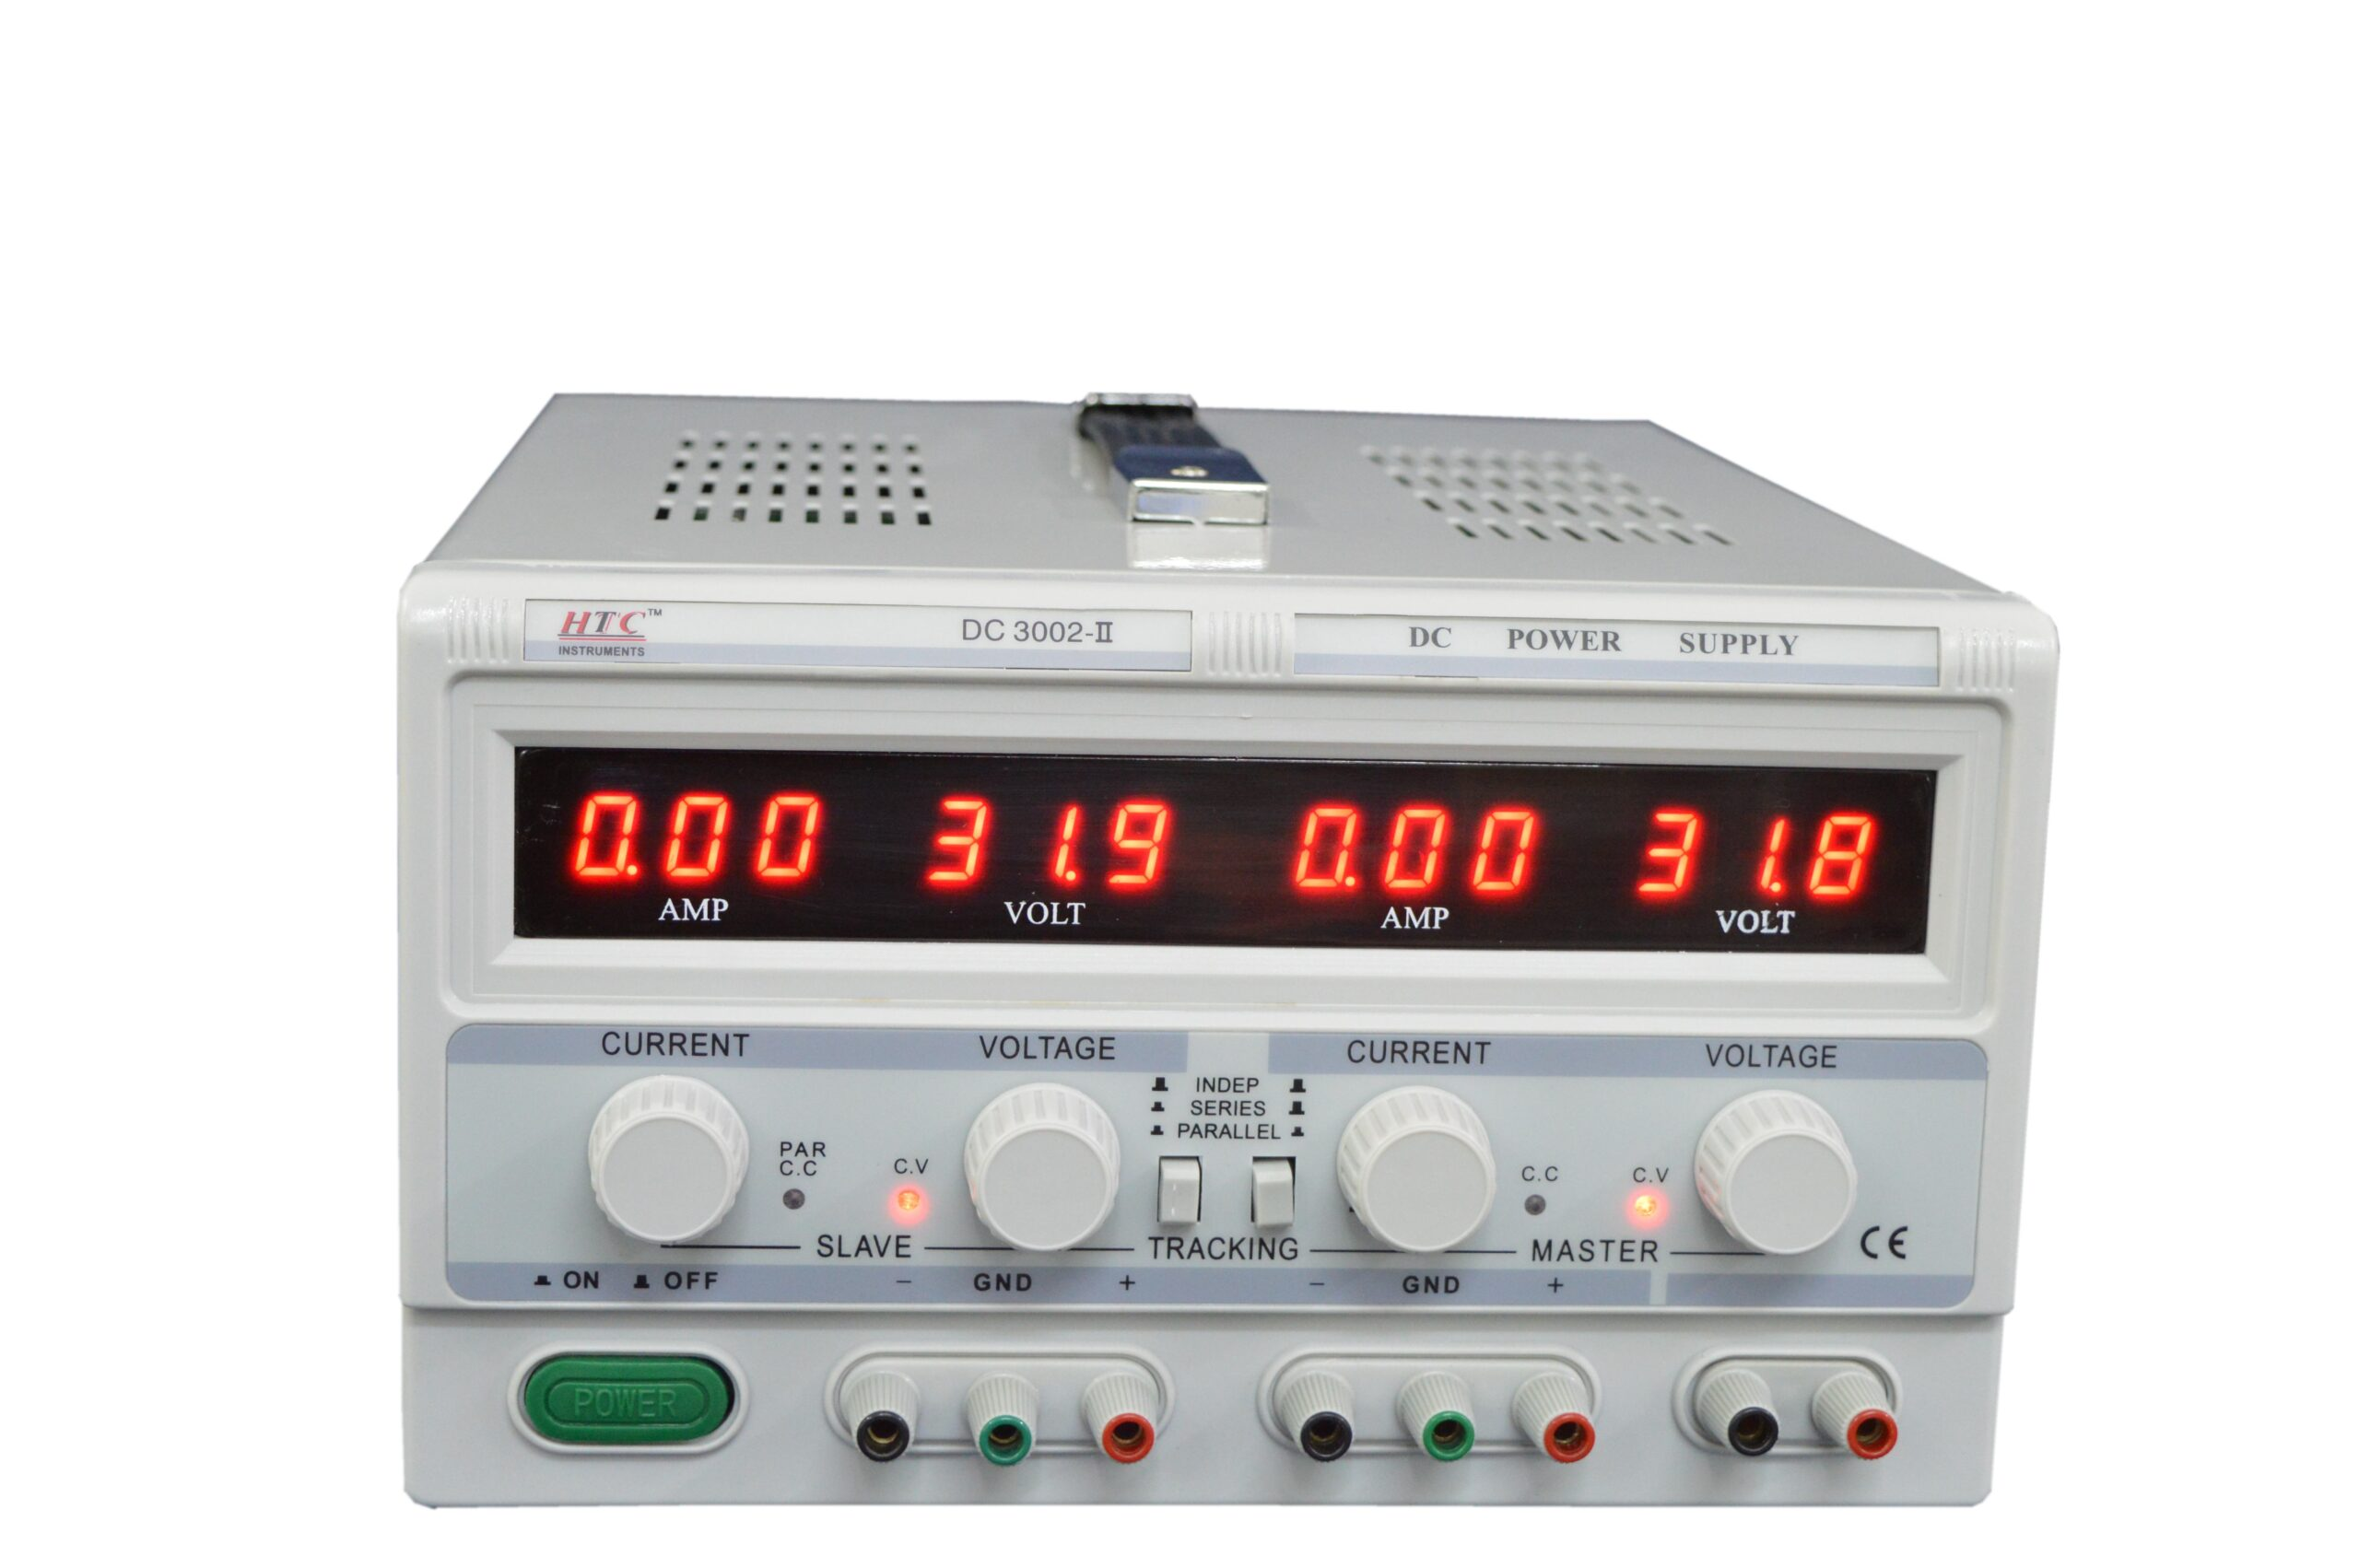
\includegraphics[width=0.5\textwidth]{./images/DC-PowerSupply.jpeg}
					\caption{DC power supply}
					\label{fig:DCPowerSupply}
				\end{figure}

			\subsubsection{Breadboard}
				A breadboard is a construction base for prototyping of electronics.A breadboard consists of plastic block holding a matrix of electrical sockets of a size suitable for gripping thin connecting wire, 
				component wires or the pins of transistors and integrated circuits (ICs). The sockets are connected inside the board, usually in rows of five sockets.

				\begin{figure}[h!]
					\centering
					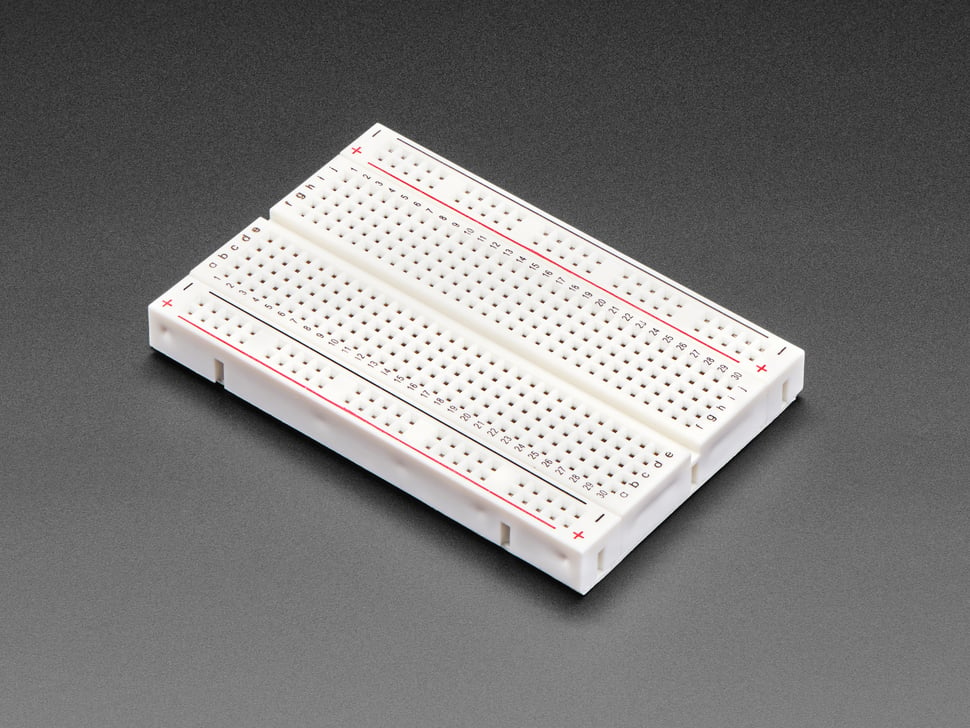
\includegraphics[width=0.5\textwidth]{images/breadboard.jpeg}
					\caption{A breadboard}
					\label{fig:breadboard}
				\end{figure}
			
			\pagebreak
			\subsubsection{Resistors}
				As stated before we needed 3 resistors for this lab report so we took 3 resistors with the proper colour code values and then we measured them and marked them.

				\begin{figure}[h!]
					\centering
					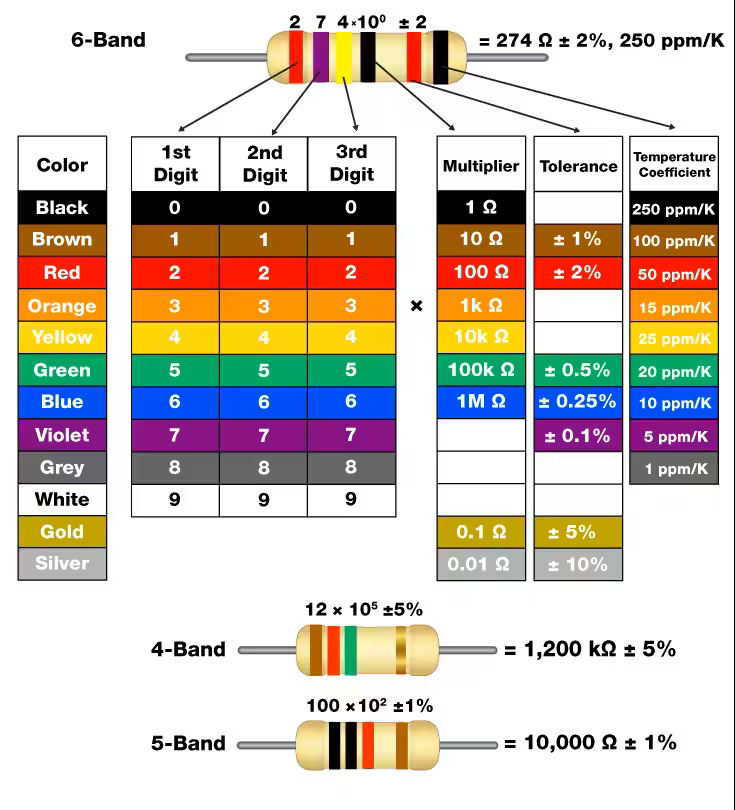
\includegraphics[width=0.35\textwidth]{images/ResistorColorCode.png}
					\caption{Resistors Color Table}
					\label{fig:ResistorsColorTable}
				\end{figure}

	
				\begin{table}[h!]
					\centering
					\begin{tabular}{@{}l|S|S@{}} % l for left, S for siunitx number column
						\toprule
						{Resistor} & {Expected Value (\si{\ohm})} & {Measured Value (\si{\ohm})} \\
						\midrule
						$R_1$ & 1000 & 988 \\
						$R_3$ & 2200 & 2142 \\
						$R_x$ & 2200 & 2169 \\
						\bottomrule
					\end{tabular}
					\caption{Expected and Measured Resistance Values}
					\label{tab:resistors}
				\end{table}

			\pagebreak
			\subsubsection{Multimeter}
				The multimeter is a versatile tool used for measuring various electrical quantities. In this lab, we will use it to measure the voltage drops across components, the currents through branches and components, and the resistance of resistors.
				To measure voltage drops, connect the multimeter in parallel across the component of interest. Set the multimeter to the voltage measurement mode and select an appropriate range.
				To measure currents, connect the multimeter in series with the branch or component. Set the multimeter to the current measurement mode and select an appropriate range.
				To measure resistance, disconnect the resistor from the circuit. Connect the multimeter probes to the resistor terminals. Set the multimeter to the resistance measurement mode and select an appropriate range.

				\begin{figure}[h!]
					\centering
					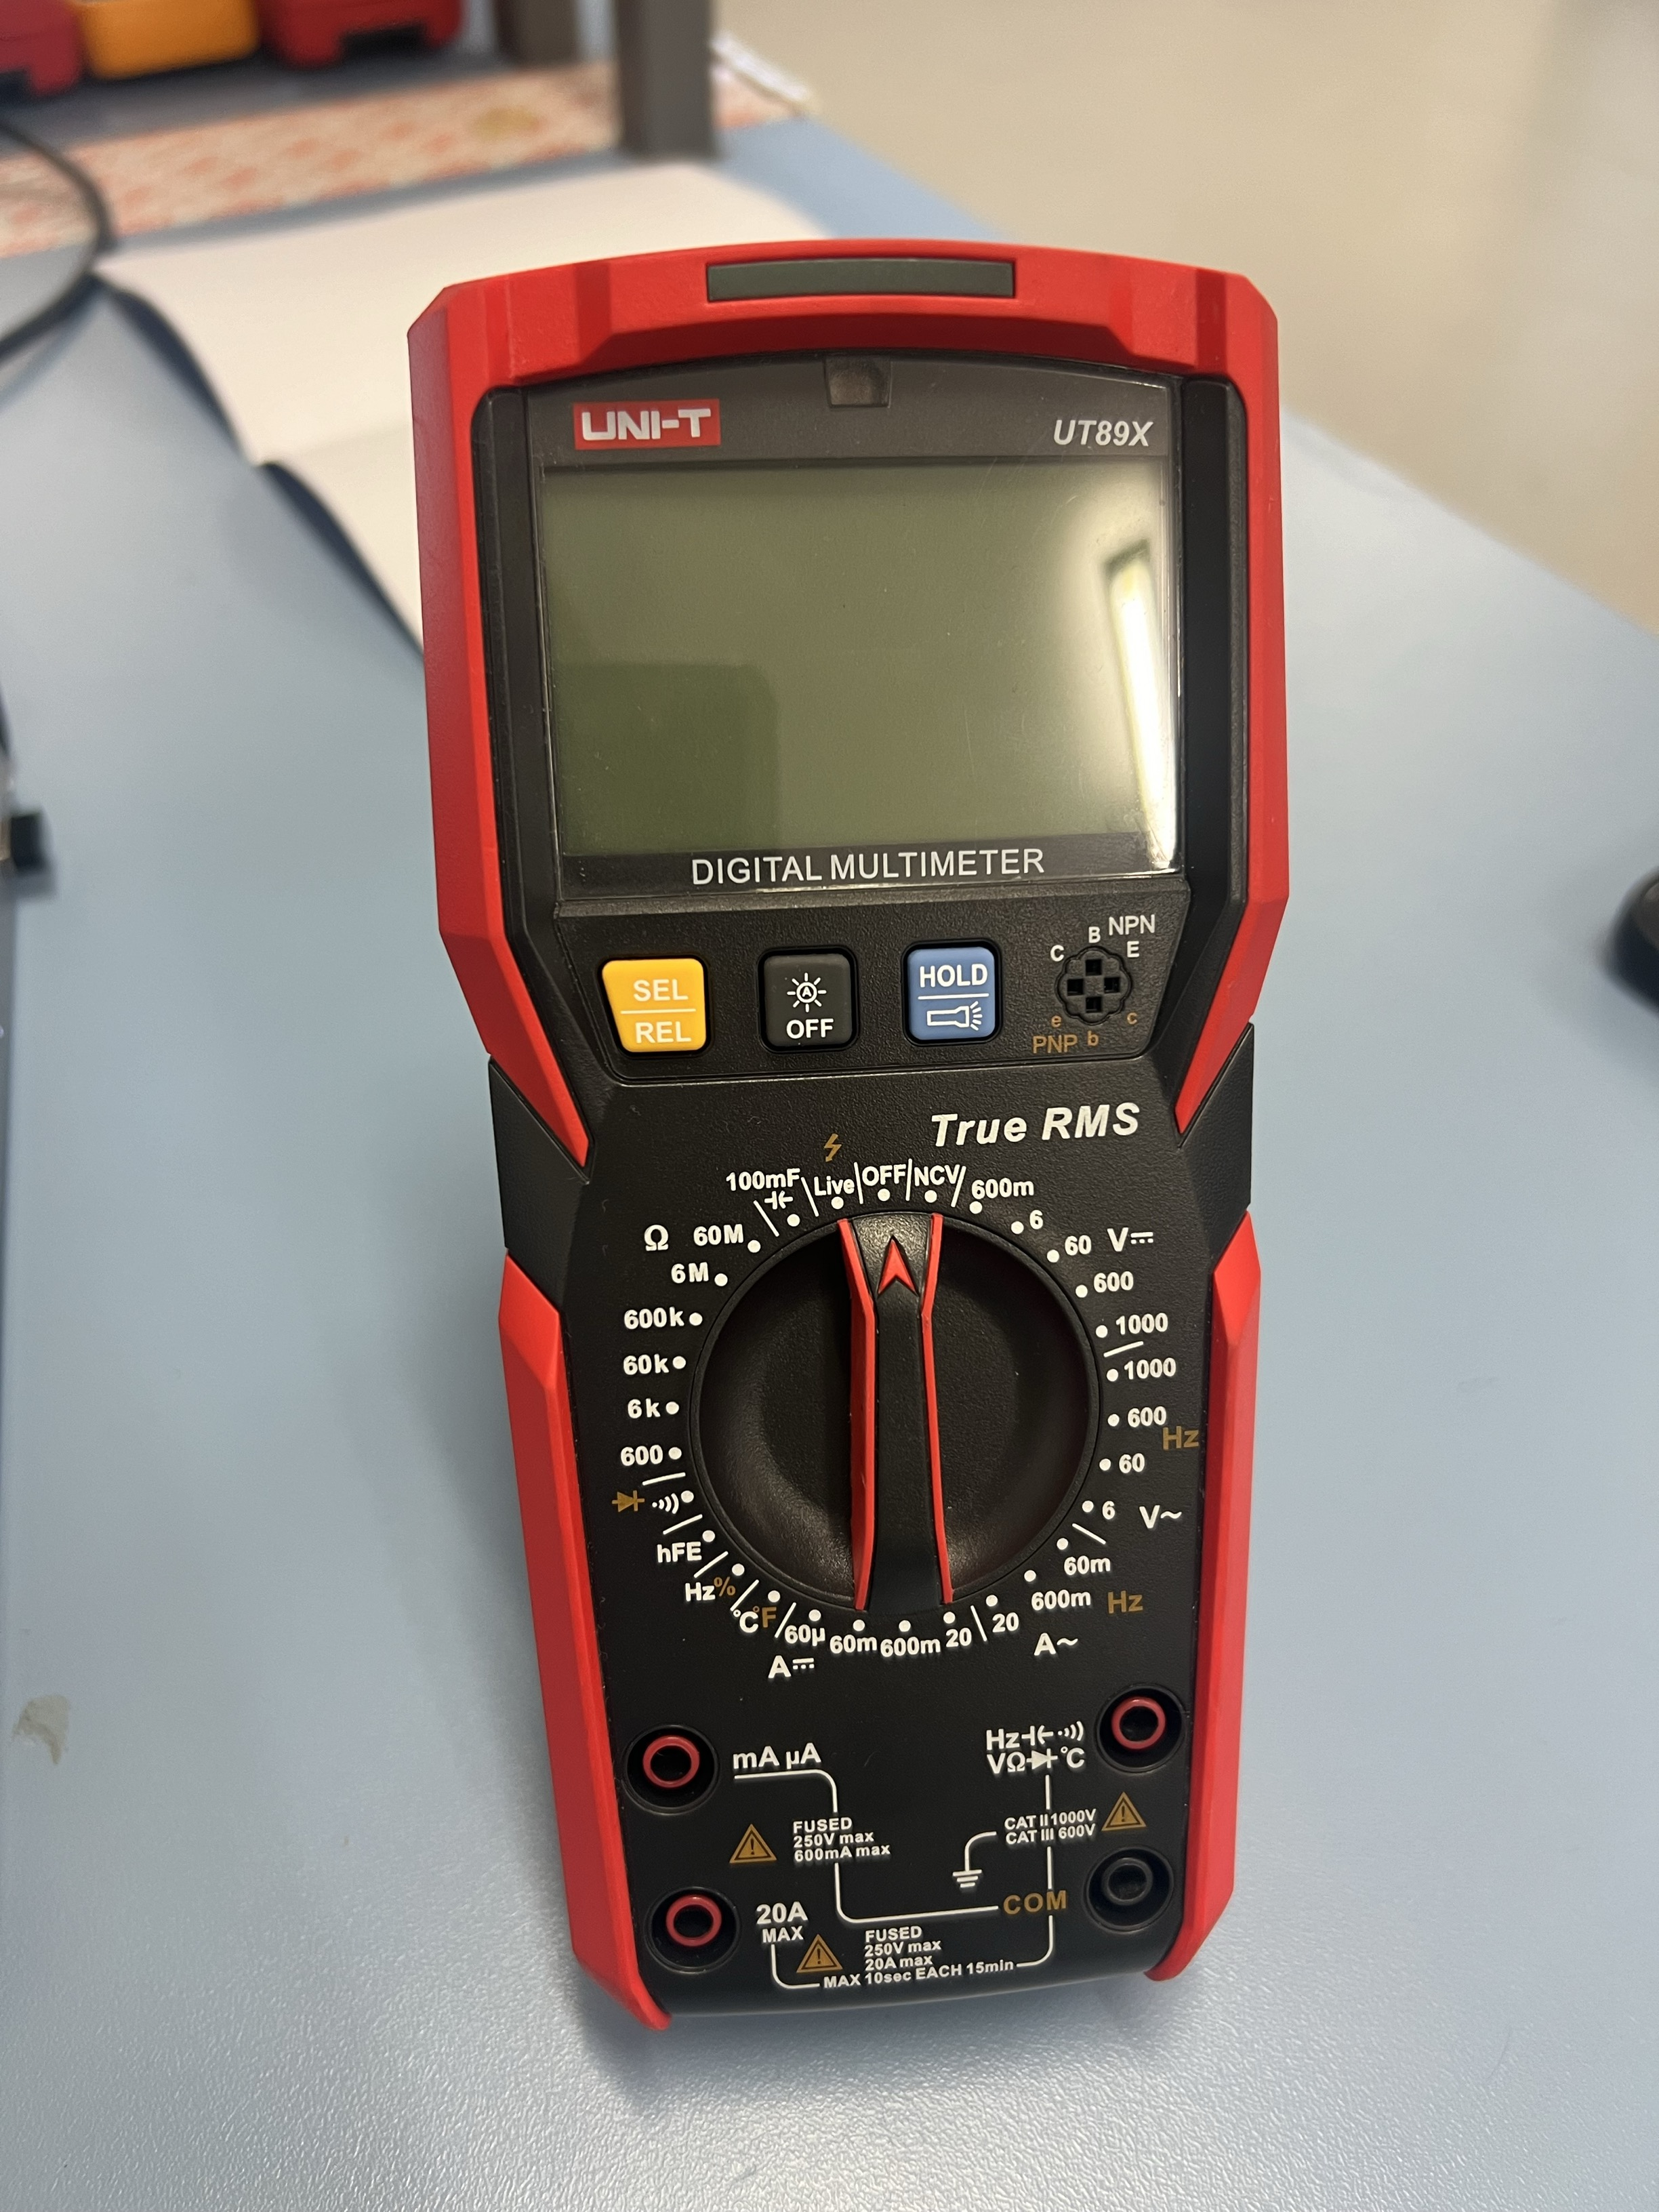
\includegraphics[height = 0.3\textheight]{images/Multimeter.jpeg}
					\caption{Multimeter}
					\label{fig:multi_meter}
				\end{figure}
			
			\subsubsection{Potentiometer}
				A potentiometer is a three-terminal resistor with a sliding ,or rotating, contact that forms an adjustable voltage divider as seen in Figure \ref{fig:potentiometer}.
				If only two terminals are used, one end and the wiper, it acts as a variable resistor.
				\begin{figure}[h!]
					\centering
					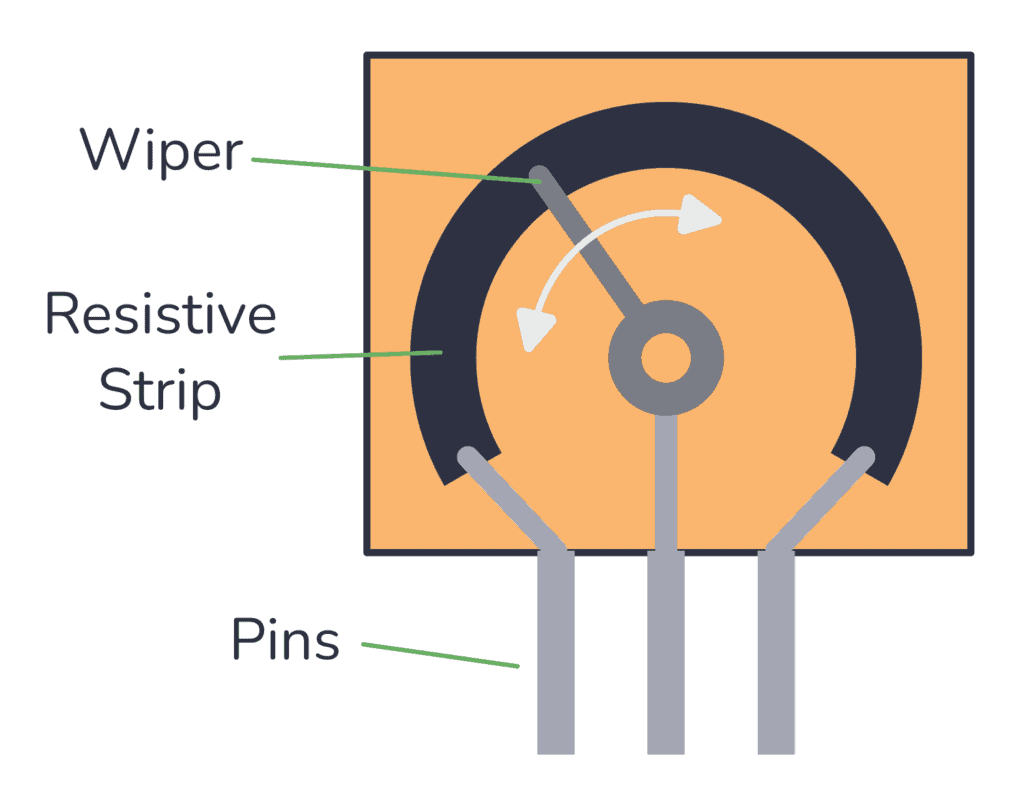
\includegraphics[width=0.5\textwidth]{images/Potentiometer.png}
					\caption{Potentiometer}
					\label{fig:potentiometer}
				\end{figure}

	\pagebreak
	\section{Procedure}
		\begin{enumerate}
			\item Connect the circuit as shown in Figure \ref{fig:wheatstone}.
			\item Set the power supply to 12V.
			\item Adjust the potentiometer and measure the voltage difference of the two nodes.
		\end{enumerate}

		\subsection{Making the Circuit}
			\begin{figure}[h!]
				\centering
				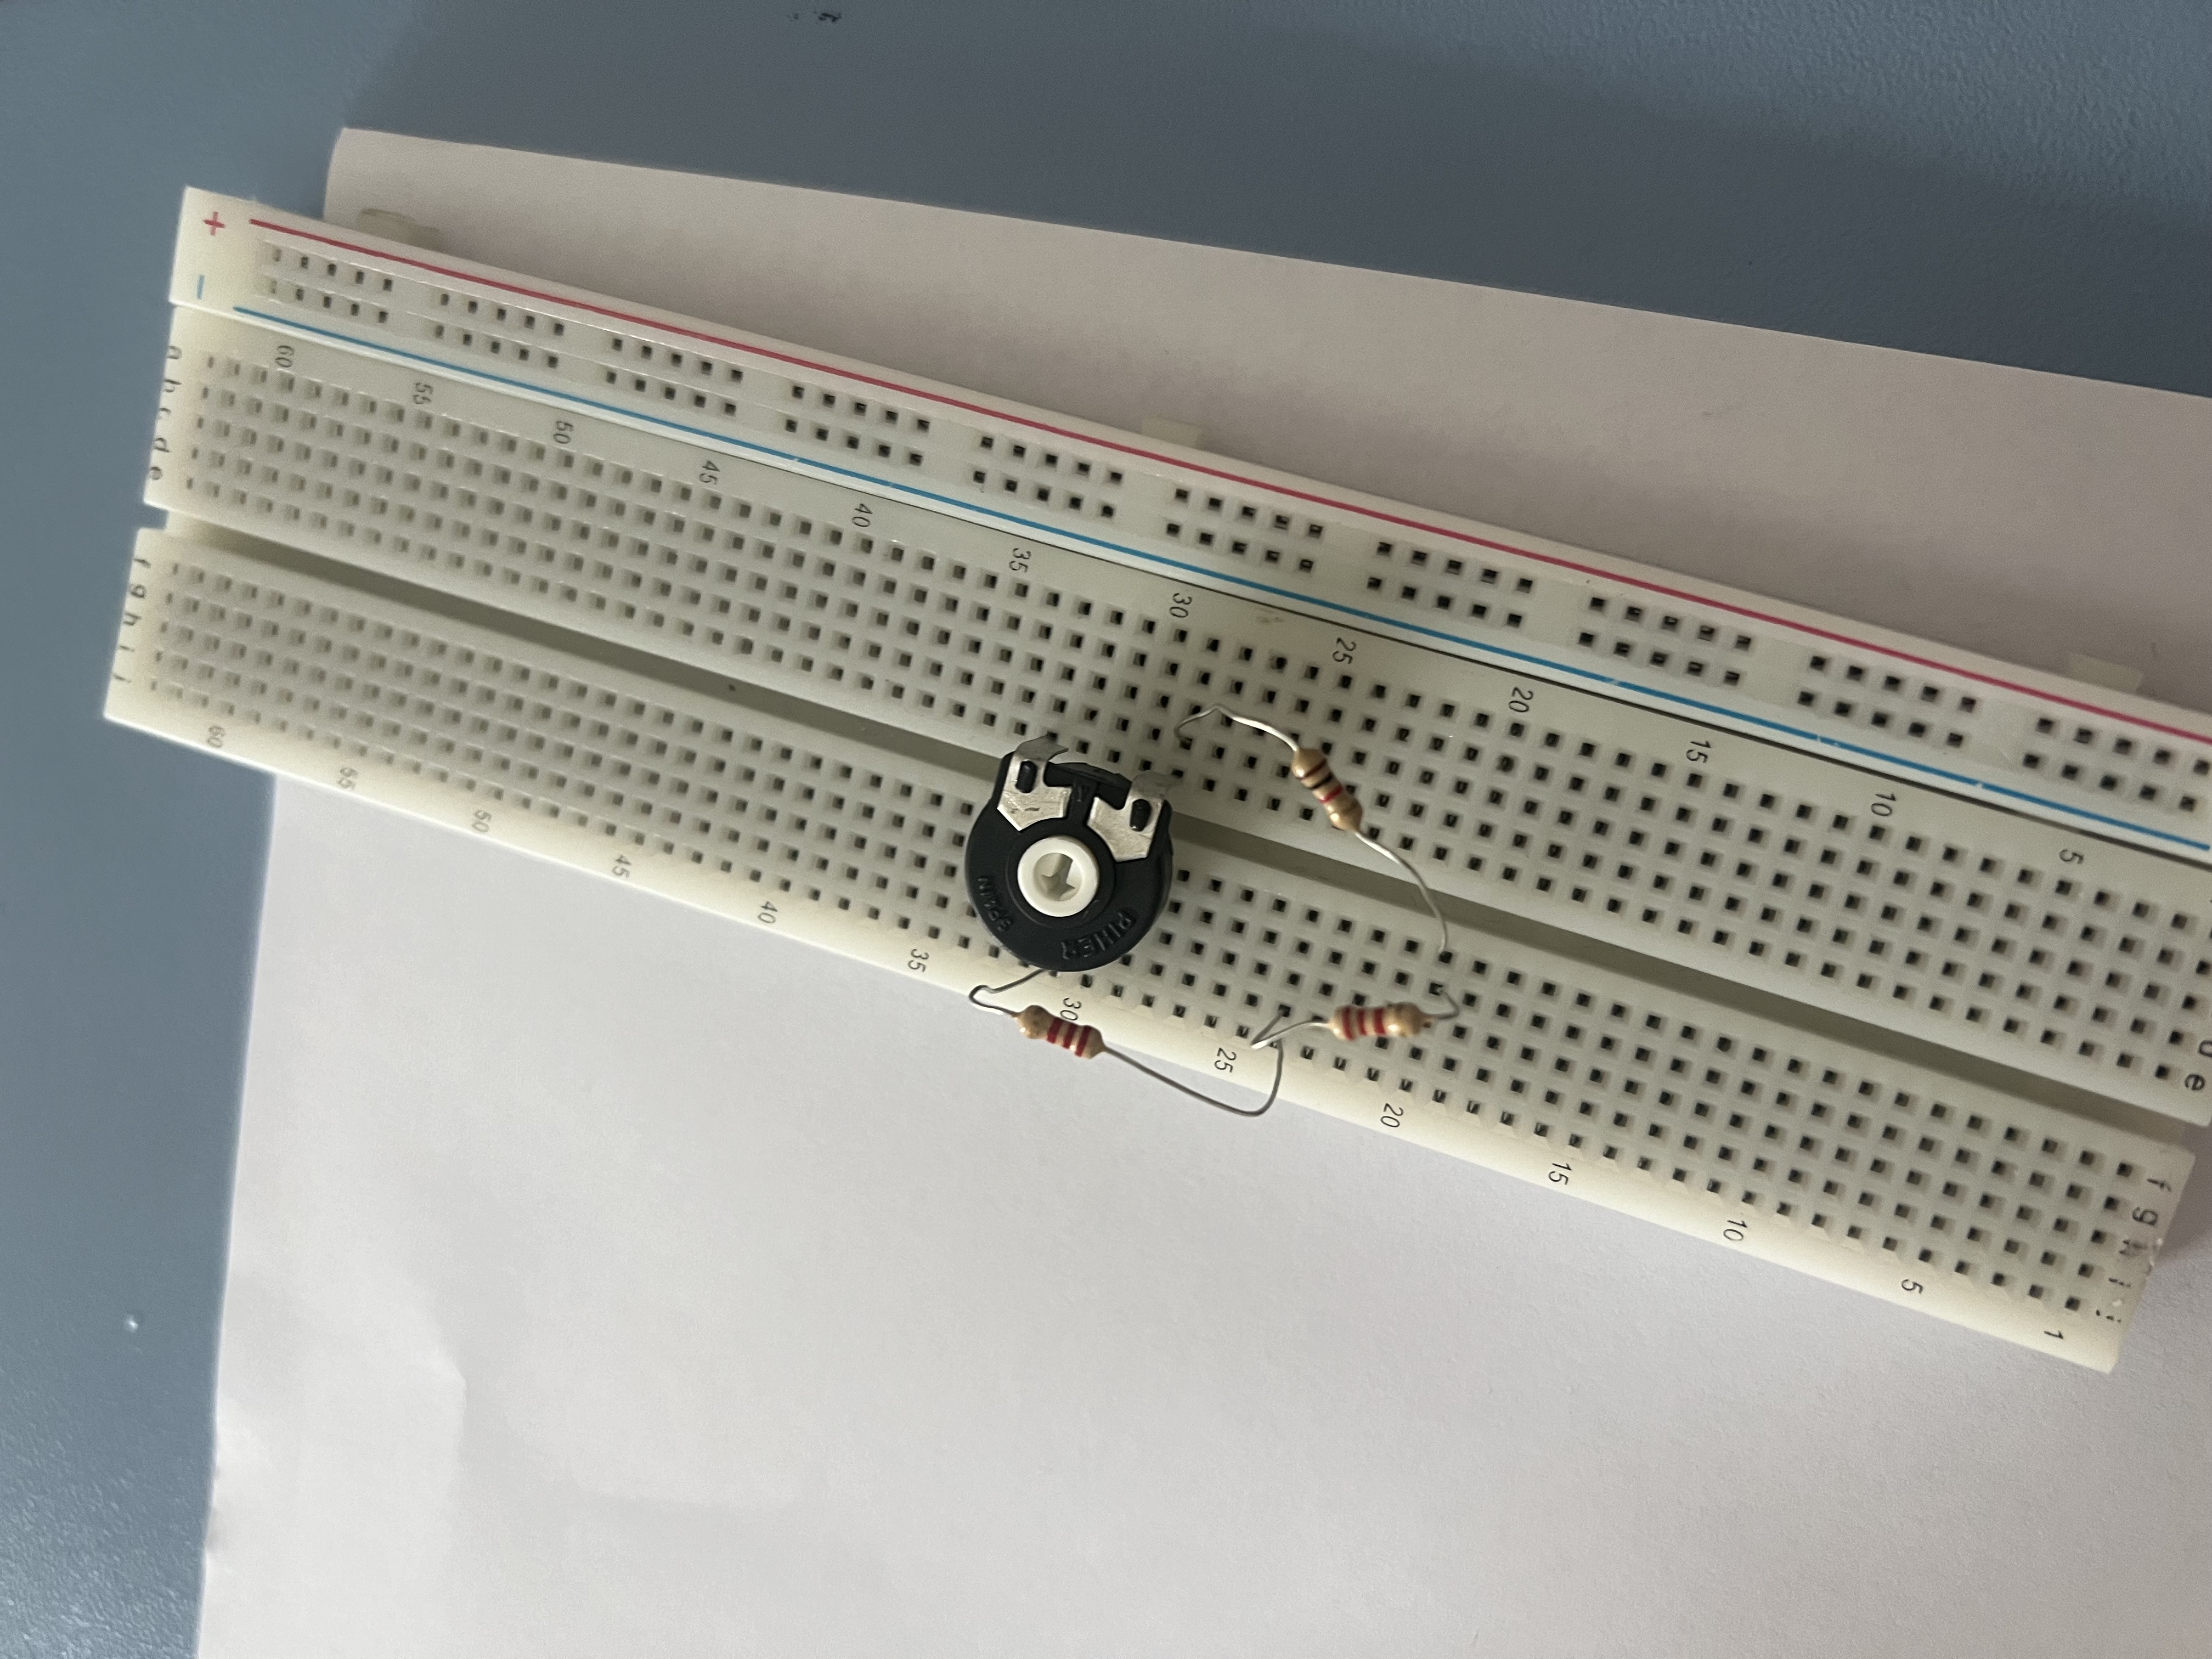
\includegraphics[width=0.5\textwidth]{images/Circuit.jpeg}
				\caption{Circuit}
				\label{fig:circuit}
			\end{figure}

			As stated before, we connected the circuit as shown in Figure \ref{fig:circuit}.
			We took two $2.2 k\si{\ohm}$ resistors and connected them in series to form one branch,
			and then we took the $1 k\si{\ohm}$ resistor and connected it in series with the potentiometer.
			We connected one pin of the potentiometer to the $1 k\si{\ohm}$ resistor and the 
			wiper to the $2.2 k\si{\ohm}$ resistor on the other branch effictively creating a wheatstone bridge.
			As we stated before in the Aparature subsection, if we just connect the potentiometer using only one
			of it it's pins and the wiper, we can use it as a variable resistor. Now all that is left is to connect
			one of the resistors to the power supply and the other to the ground, making sure that
			either the 2.2 $k$\si{\ohm} resistor or the potentiometer is connected to the ground,
			and the other two to the power supply.
			
		\subsection{Calculation}
			To calculate $V_{db}$ first we have to calculate $V_{d}$ and $V_{b}$.
			Luckly we have a tool for calculating the voltage drop across ressistors called the voltage dividor formula.
			Using the voltage dividor formula we can calculate the voltage drop across the $2.2 k\si{\ohm}$ resistor,
			which would give us the $V_b$, and then we can calculate the voltage drop across the $1 k\si{\ohm}$ resistor
			which would give us the $V_d$. Then we can calculate the $V_{db}$ by subtracting $V_d$ from $V_b$.

			\begin{align*}
				V_{b} &= 12 \times \frac{R_x}{R_x + R_3} \\
				V_{d} &= 12 \times \frac{R_2}{R_1 + R_2} \\
				V_{db} &= V_{d} - V_{b}
			\end{align*}

			In our case we know what $R_x$ is, and that it is constant; so we have that $V_b$ is constant, and we can calculate it
			\begin{equation*}
				V_{b} = 12 \times \frac{2200}{2200 + 2200} = 6 V
			\end{equation*}
		
		\pagebreak
		\subsection{Measuring the Voltage}
			To measure the voltage drop across the two nodes, we connected the multimeter in parallel with the two nodes.
			We will just change the value of the potentiometer and measure the voltage drop across the two nodes,
			one being the input of the potentiometer and the other being the input of the $2.2 k\si{\ohm}$ resistor $R_x$.
			\begin{figure}[h!]
				\centering
				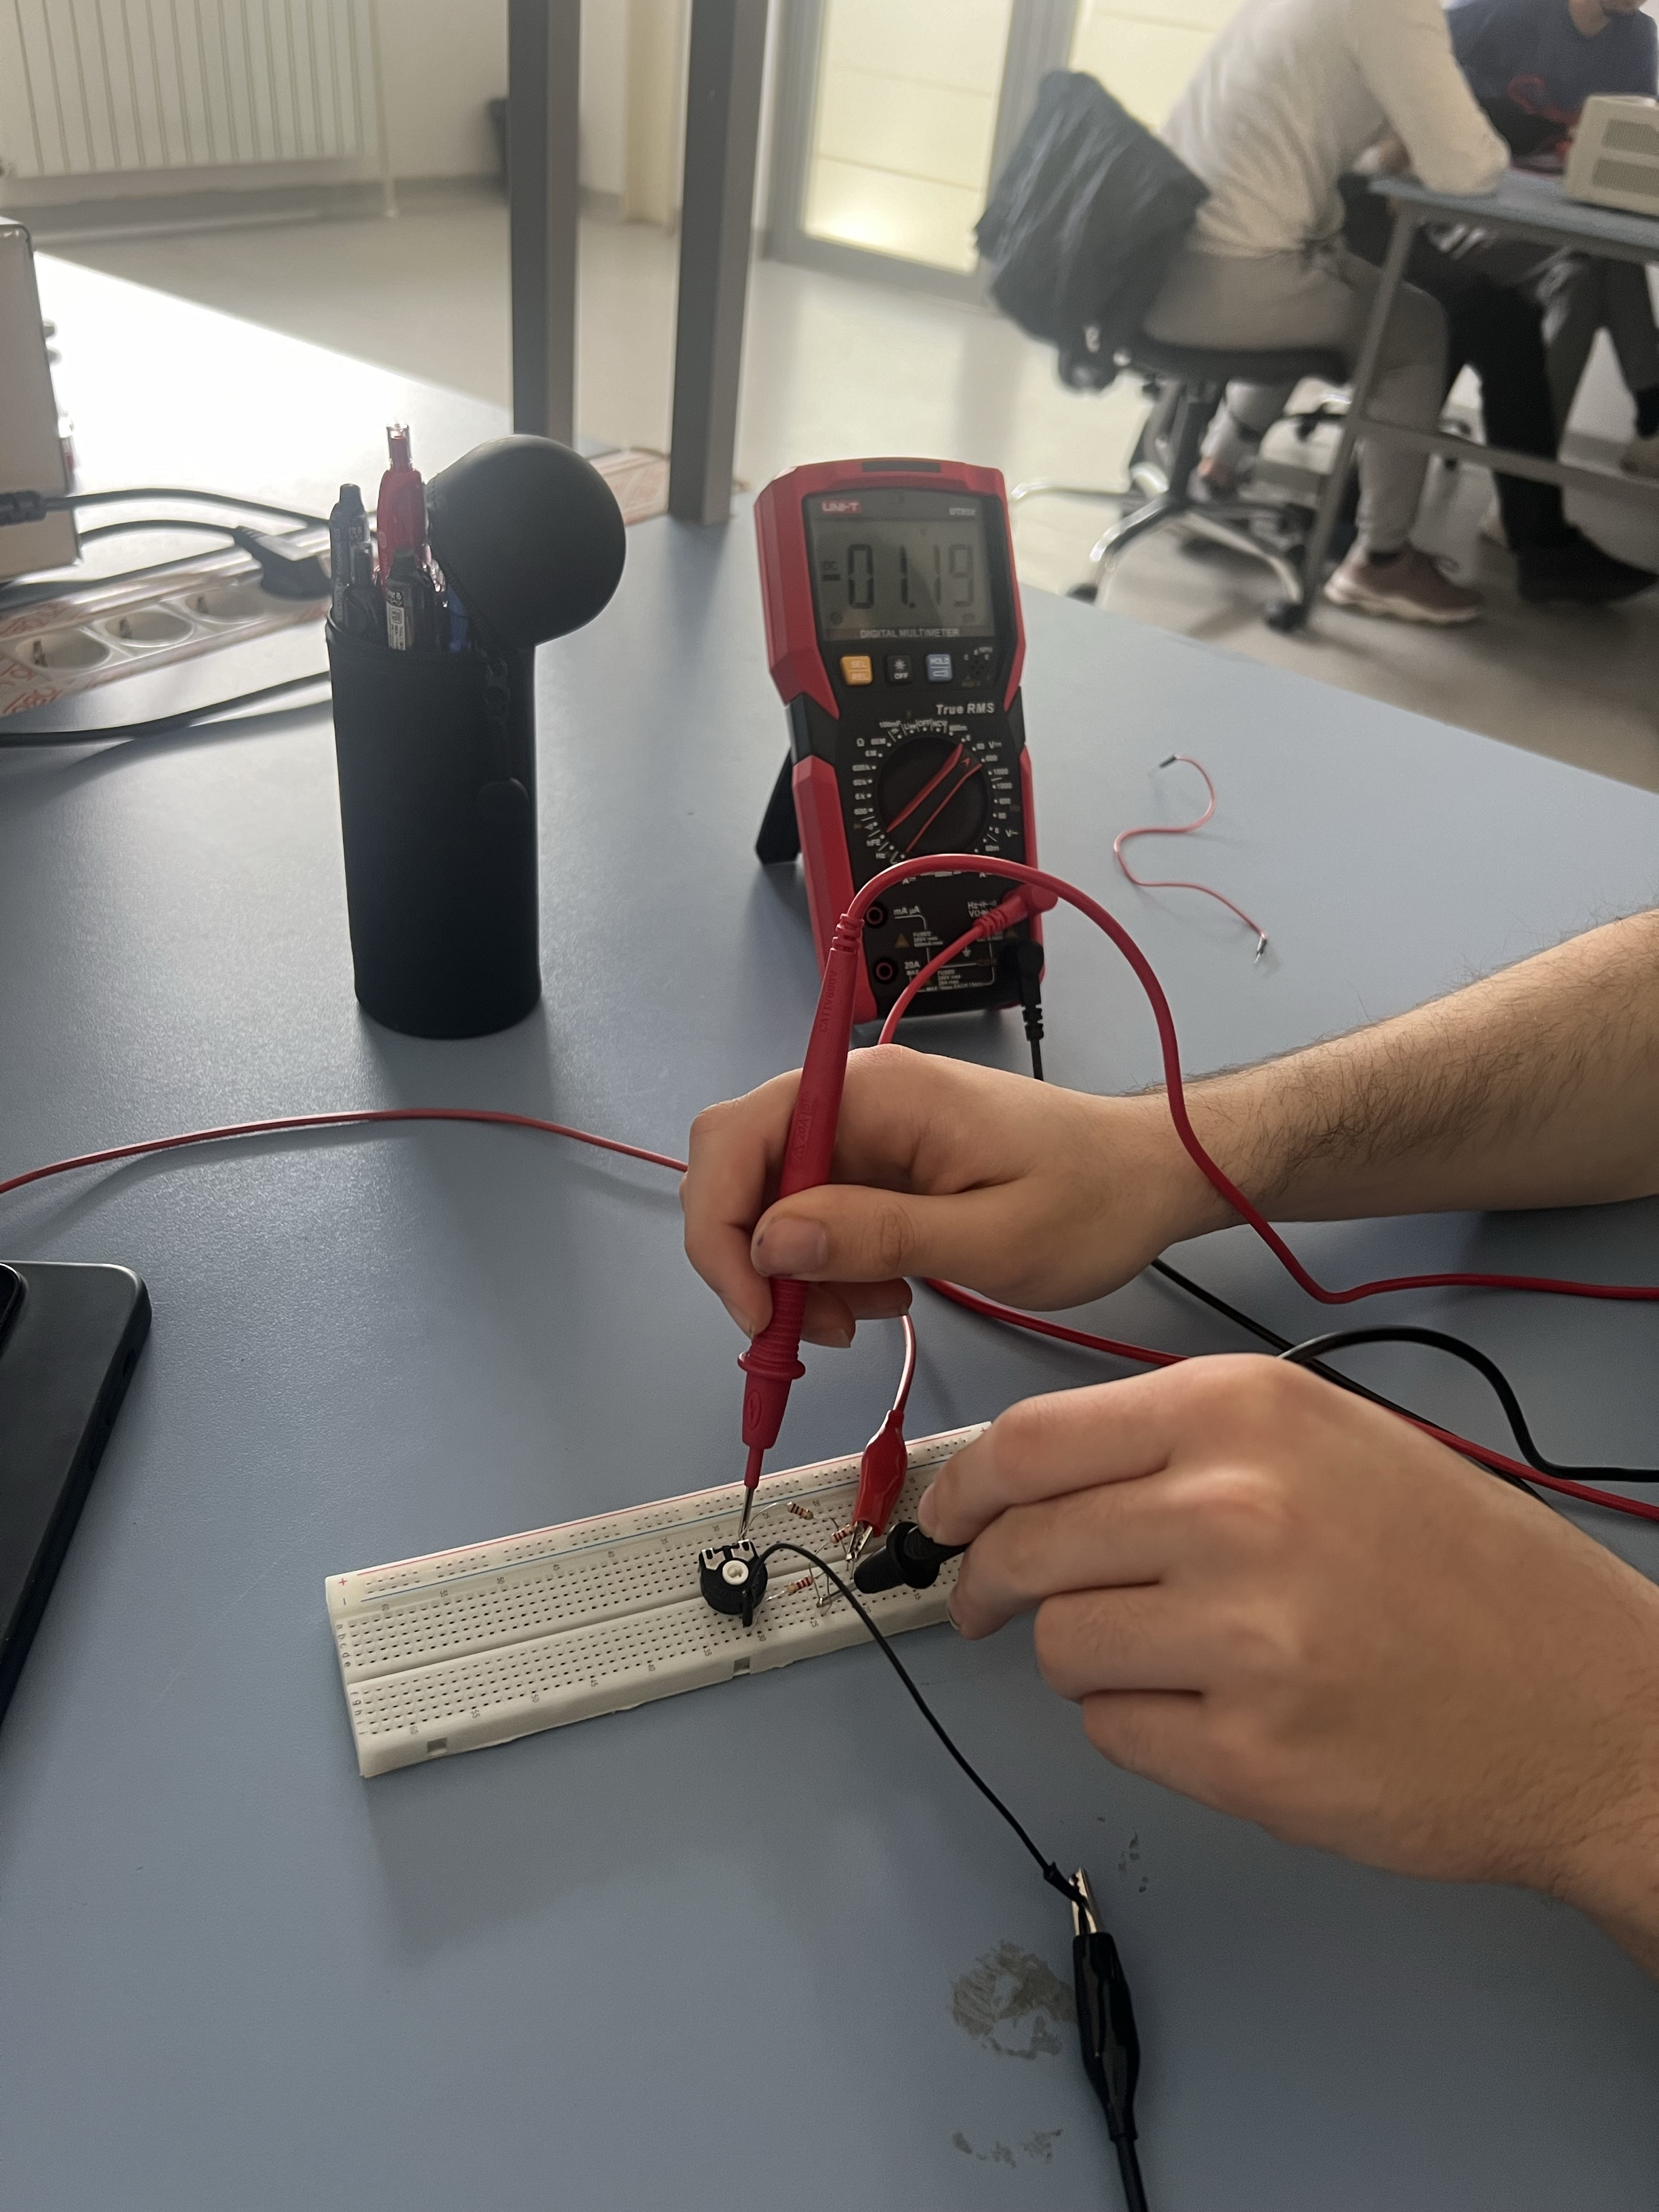
\includegraphics[width=0.5\textwidth]{images/MeasuringVoltage.jpeg}
				\caption{Measuring Voltage $V_{db}$}
				\label{fig:multi_meter}	
			\end{figure}

		\subsection{Results}
			Now that everything is explained, since they are way to many measurements we will not provide ALL the images
			that there were to show but just the meaasurements and calculations that we did.

			\begin{table}[ht]
				\centering
				\begin{tabular}{|c|c|c|c|c|c|c|c|c|c|c|c|}
					\hline
					R ($\Omega$) & 500 & 600 & 700 & 800 & 900 & 1000 & 1100 & 1200 & 1300 & 1400 & 1500 \\ \hline
					$V_{ab}$ measured & -1.73 & -1.19 & -0.65 & -0.15 & 0.23 & 0.60 & 0.32 & 0.56 & 0.83 & 0.99 & 1.20 \\ \hline
					$V_{ab}$ calculated & -2.0 & -1.5 & -1.06 & -0.67 & -0.32 & 0.00 & 0.29 & 0.55 & 0.78 & 1.00 & 1.20 \\ \hline
				\end{tabular}
				\caption{Measured and calculated values of $V_{ab}$ for varying R.}
				\label{tab:my_label}
			\end{table}

			A quick note, whilst doing this lab we noticed that the potentiometer was not working properly, 
			the wiper of the potentiometer was not making proper contact with the resistive material and was wobbly.
			We tried to fix it but we could not, so we had switch the potentiometer, because of this we see that
			the measured voltage decreases as expected from 500 to 800, but then it starts to increase again
			up to 1000 and then here we swapped it for a better one where we started to see better results.
			In reality the 800 \si{\ohm} resistance that we measured was actually something around 1000 \si{\ohm}.
			Sadly due to the lack of time we were not able to measure the voltage drops with the new potentiometer.

	\pagebreak
	\section{Conclusion}
			Here we have seen the balance of the wheatstone bridge, and when it happense.
			We also saw what happense when we aproach the balance point.
			In the end we saw that when we got the potentiometer and the 1k \si{\ohm} resistor to be equal,
			making their ratio 1 to 1 just like the 2.2 \si{\ohm} resistors, the bridge was balanced.

			\vspace{5mm}

			We also learned what a potentiometer is, and how to use it as a variable resistor, or more generally how
			to use it.
\end{document}
